
%=============================================================================%

% Erstes Inhaltsverzeichnis

\frame{
	\frametitle{Inhaltsverzeichnis}
	\small
	\tableofcontents
	\normalsize
}

%=============================================================================%

% Eine Grafik in einer Figure darstellen.

\section{Eine Grafik}

\begin{frame}
 
  \begin{figure}[h]
  \begin{center}
	  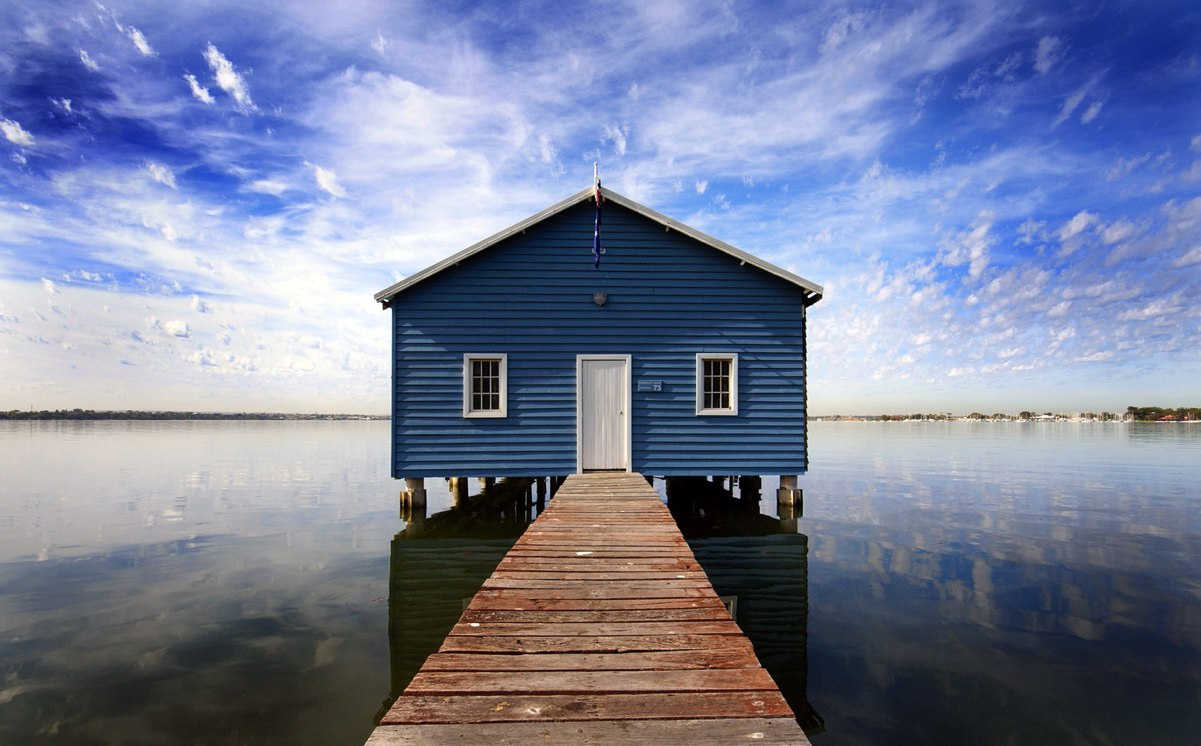
\includegraphics[width=0.8\textwidth]{figures/back.jpg}
  \end{center}
  \caption{ Caption der Grafik }
  \label{fig:openni}
  \end{figure}
  
\end{frame}


%=============================================================================%

%Etwas spaltenweise anzeigen

\section{zwei Spalten}

%Ein Inhaltsverzeichnis zur Übersicht
\frame{
	\frametitle{Inhaltsverzeichnis}
	\small
	\tableofcontents[currentsection,hideothersubsections]
	\normalsize
}

%Zwei Spalten mit 55 und 45 Prozent des Bildschirms
\begin{frame}
  \begin{columns}
        \column{.55\textwidth}
                \pgfimage[width=\textwidth]{figures/back.jpg}
		\newline Ein Text unter dem Bild
        \column{.45\textwidth}
                \begin{enumerate}
                \item Föhr
                \item Fähr
                \end{enumerate}
\end{columns}

\end{frame}

%=============================================================================%

\section{Blocktext}

\begin{frame}[t]
    \begin{block}{Blocktitel}
        Blocktext
  \end{block}

  \begin{exampleblock}{Beispielblocktitel}
        Beispielblocktext
  \end{exampleblock}

  \begin{alertblock}{Warnungsblocktitel}
        Warnungsblocktext
  \end{alertblock}
\end{frame}

%=============================================================================%

\section{Nacheinander einfügen}

\begin{frame}

  \begin{itemize}
	  \item Einleitung
	  \item<2-> daher
	  \item<alert@3> aber Achtung!
	  \item<3-> also so und so
	  \item<4-> Schlussfolgerung
	  \item<5|alert@3> Nun Aber
  \end{itemize}

\end{frame}


%=============================================================================%

\subsection{Noch ein weiterer Test}

\frame[<+->][label=Liste]{
	\frametitle{"Uberschrift}
	\begin{itemize}
	\item uno
	\item duo
	\end{itemize}
}

%=============================================================================%

% Ergänzung zu Frames

% \begin{frame}[Overlay-Aktionen][Optionen]{Titel}{Untertitel}
% 	Inhalt
% \end{frame}
% 
% Der (grüne) Teil nach \begin{frame} ist optional und muss daher nicht angegeben werden. Alternativ zur Frame-Umgebung kann man eine Folie auch mittels \frame{} Befehl erstellen, welcher als Parameter den Frameinhalt entgegen nimmt. Als Frameinhalt sind weitere LaTeX-Umgebungen erlaubt, solange sie die Zeichenkodierung nicht ändern. Es sei denn die fragile Option ist gesetzt.
% 
% Overlay-Aktionen
%     Overlay-Aktionen setzen die Standard-Overlay-Aktionen aller Umgebungen innerhalb des Frames, welche Aktion-Spezifikationen erlauben. Dazu gehören u.a. \item bei Listen und Block-Umgebungen.
% 
%     <+->
%         Sorgt dafür, dass die Elemente stückweise zum Vorschein kommen.
% 
% Optionen
% 
%     allowdisplaybreaks
%         Sorgt durch Aufruf von \allowdisplaybreaks aus AMS-LaTeX für einen Seitenumbruch bei mehrzeiligen Formelumgebungen. Funktioniert nur im Zusammenhang mit der Option allowframebreaks
%     allowframebreaks
%         Passt der Inhalt nicht mehr auf ein Slide, wird er automatisch auf mehrere Slides verteilt. Allerdings ist somit kein Overlay mehr möglich.
%     b,c,t
%         Sorgt dafür, dass der Frame nach unten (b), zentriert (c) oder nach oben (t) ausgerichtet wird.
%     fragile
%         Wird für Quelltextumgebungen, z.B. verbatim, benötigt.
%     label=name
%         Legt einen Namen für ein Frame fest um es später mit \againframe{name} erneut aufrufen zu können.
%     plain
%         Unterdrückt die Anzeige der Überschrift, Fußzeile und Sidebar.
%     squeeze
%         Verkleinert die vertikalen Abstände so weit wie möglich um u.U. mehr auf der Folie unterbringen zu können




